\section{C\#}

C\# — це сучасна об’єктно-орієнтована мова програмування загального призначення, розроблена корпорацією Microsoft у рамках її ініціативи .NET і пізніше затверджена як стандарт Європейською асоціацією виробників комп’ютерів (ECMA) і міжнародними стандартами (ISO). В основному C\# використовується для розробки Web додатків, ігор та застосунків для Windows. Розгляньмо деякі із бібілотек.

\subsection{Використання GNU GMP бібліотеки із мовою програмування С\#}

Як вже було згадано вище, GNU GMP допомагає виконувати будь які арифметичні операції із довільною точністю, що обмежена лише пам'яттю машини, на якій виконується программа. Для того, щоб використовувати цю бібліотеку в мові програмування СSharp слід встановити до проєкту Nuget пакет із назвою "Math.Gmp.Native.NET".

Бібліотека "Math.Gmp.Native.NET" автоматично завантажує на виконання 32-бітну або 64-бітну бібліотеку GNU MP, яка відповідає поточній архітектурі центрального процесора, тим самим дозволяючи будувати проекти Visual Studio для режимів Any CPU, x86 або x64. Вона базується на розширеній збірці GNU MP, яка автоматично визначає тип поточного процесора і вибирає оптимізацію коду на мові асемблера для даного процесора, тим самим забезпечуючи найкращу продуктивність. 

Клас Math.Gmp.Native.gmp\_lib містить статичний метод для кожної з функцій GNU MP. Інші типи визначені для відтворення структур і псевдонімів типів GNU MP і мов C, а також мовних конструкцій C.

Заради зручності цю довідку було створено з офіційного посібника GNU MP версії 6.1.2. Вона демонструє, з прикладами, як кожна функція GNU MP викликається в .NET.

Для початку порівняємо код мовою програмування C\# із кодом на Rust.(рис. 1)

\begin{figure}[!h]
     \centering
     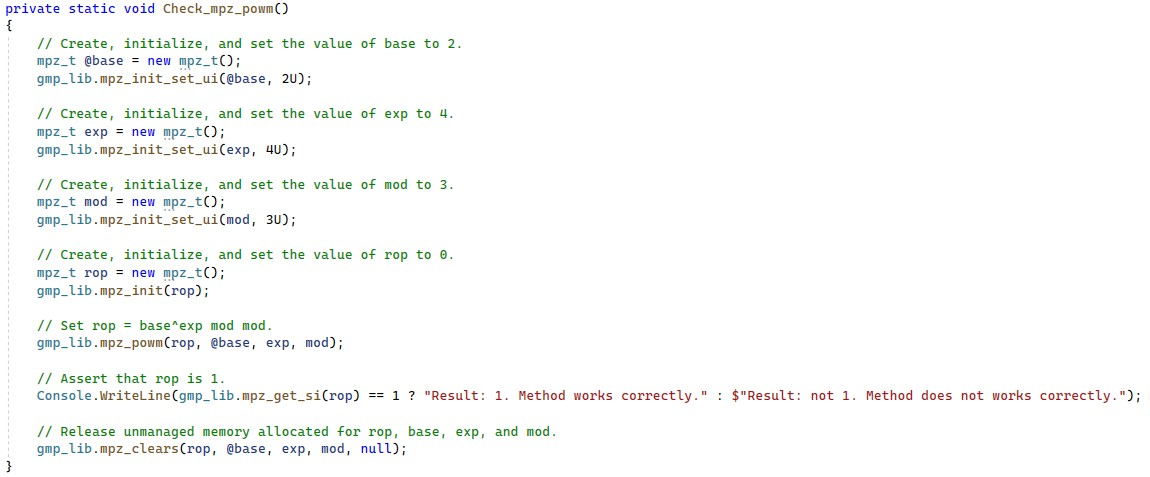
\includegraphics[scale = 1]{../IMAGES/image_01_c_sharp_lab_01.jpg}
     \caption{Приклад піднесення до степеня.}
     \label{fig:}
\end{figure}

Видно, що для використання GMP треба використати змінні класу mpz\_t і задавати певні значення чисел у функцію mpz\_pown. Якщо метод відпрацював успішно, то в консолі можна буде побачити повідомлення про коректну роботу. (рис. 2)

\begin{figure}[!h]
     \centering
     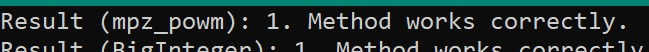
\includegraphics[scale = 1]{../IMAGES/image_02_c_sharp_lab_02.jpg}
     \caption{Приклад для перевірки коректності роботи алгоритму.}
     \label{fig:}
\end{figure}

Розглянемо для остаточного розуміння, як саме використовувати написану мовою програмування C бібліотеку у поєднанні із СSharp оболонкою для знаходження зворотнього елементу. (рис. 3)

\begin{figure}[!h]
     \centering
     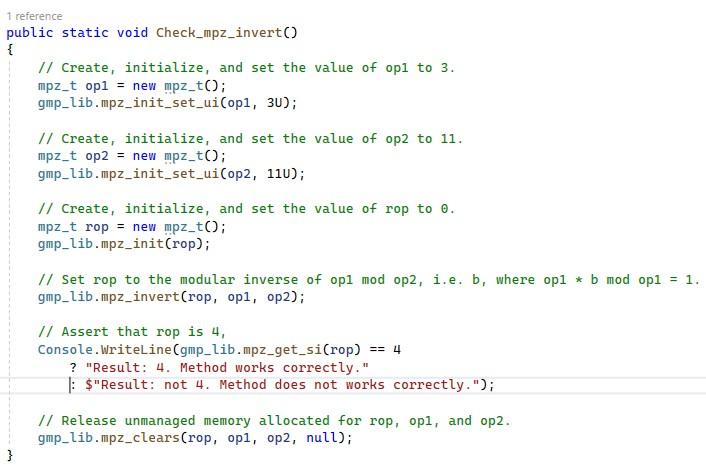
\includegraphics[scale = 1]{../IMAGES/image_05_c_sharp_lab_05.jpg}
     \caption{Приклад знаходження зворотнього елементу.}
     \label{fig_05:}
\end{figure}

\newpage
\par

\subsection{Використання System.Numerics.BigInteger бібліотеки із мовою програмування C\#}

BigInteger - це тип даних в програмуванні, який дозволяє представляти та виконувати операції з великими цілими числами, які виходять за межі можливостей стандартних числових типів. В інших мовах програмування цей тип може мати різні назви, але концепція залишається однаковою - він дозволяє працювати з числами довільної довжини і не обмежується розміром пам'яті, яку може займати число.

У .NET BigInteger знаходиться в просторі імен System.Numerics і забезпечує можливість виконувати арифметичні операції, порівнювати та взаємодіяти з великими цілими числами, незалежно від їх розміру, забезпечуючи точність та надійність операцій. Це особливо корисно при виконанні обчислень, де великі числа можуть виникати при розв'язанні математичних задач, криптографії, обробці великих даних тощо.

Таким чином, маємо реалізацію піднесення до степеню, використовуючи System.Numerics.BigInteger.ModPow.

\begin{figure}[!h]
     \centering
     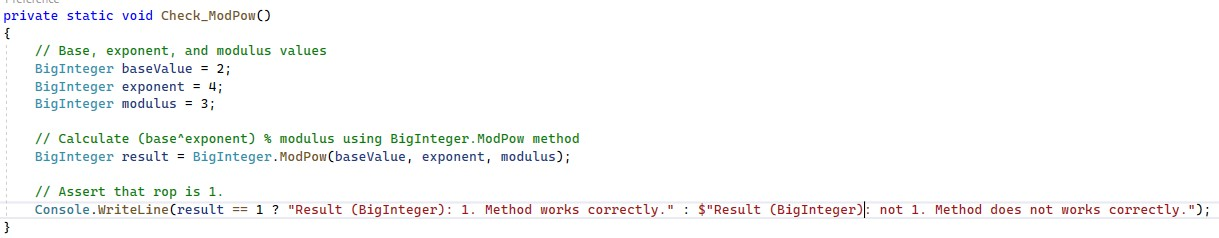
\includegraphics[scale = 1]{../IMAGES/image_03_c_sharp_lab_03.jpg}
     \caption{Приклад піднесення до степеня BigInteger.}
     \label{fig_03:}
\end{figure}

Після виконання такого шматочку коду в результаті побачимо

\begin{figure}[!h]
     \centering
     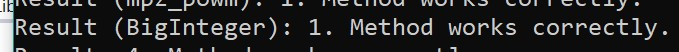
\includegraphics[scale = 1]{../IMAGES/image_04_c_sharp_lab_04.jpg}
     \caption{Результат піднесення до степеня BigInteger.}
     \label{fig_04:}
\end{figure}

Таким чином, бачимо, що обидві функції коректно працюють.


\subsection{Висновки до розділу C\#}

Мова програмування C\# є відмінним вибором для роботи із різними арифметичними операціями, оскільки вона підтримує різні бібліотеки для роботи з великими числами та арифметикою високої точності. Перш за все, вбудований клас System.Numerics.BigInteger надає можливість оперувати дуже великими цілими числами без втрати точності, що робить його ідеальним вибором для обчислень, де великі числа важливі.

Додатково, наявність зовнішніх бібліотек, таких як Math.Gmp.Native або System.Numerics.MPFR, розширює можливості C\#. Ці бібліотеки забезпечують швидку та ефективну роботу з великими числами, що особливо корисно для вимогливих до продуктивності застосувань. Наприклад, вони можуть бути використані в задачах криптографії, математичних моделях або статистичних розрахунках, де точність та продуктивність є ключовими.

Крім того, можливість використання різних бібліотек дає можливість вибору відповідно до конкретних потреб проекту. Наприклад, System.Numerics.BigInteger надає зручний та простий інтерфейс для роботи з великими числами, тоді як Math.Gmp.Native або System.Numerics.MPFR можуть бути використані для оптимізації продуктивності у вимірюваних додатках.

Загалом, здатність C\# підтримувати і вбудовані, і сторонні бібліотеки для роботи з арифметичними операціями робить її потужним і гнучким інструментом для вирішення широкого спектру математичних завдань у сучасному програмуванні.


